\chapter{Methoden}\label{ch:method}
Um die nachfolgenden Methoden zur Analyse und Visualisierung von Datenqualität zu vergleichen, werden sowohl qualitative als auch quantitative Untersuchungen durchgeführt.
Für eine Datenqualität, die sich in einem Unternehmen etablieren kann, ist es nötig diese von den Gesichtspunkten aller Stakeholdern zu betrachten.
Anhand einer Stakeholderanalyse wird es möglich sein die Probleme der Datenqualität auf zwei Ebenen zu betrachten. 
Zum einen benötigen die Business-User gute Datenqualität, um die richtigen Zinsen anhand des Risikoscorings zu vergeben und auf der anderen Seite benötigen die Entwickler eine Möglichkeit, um ihre ETL-Strecken zu überprüfen.
Für diese beiden Probleme können zwei verschiedene Verfahren eingesetzt werden.
Zur Identifikation und Überprüfung des Risikoscores kann ein Machine Learning Algorithmus trainiert werden, der die korrekten Werte vorhersagt und somit einen Aufschluss darüber gibt, wie viele Datensätze aktualisiert werden sollten.
Um die ETL-Strecken zu analysieren sind die Metadaten zu den Prozessen nötig, die anzeigen, wie viele Daten an jedem Tag extrahiert wurden. 
Auffälligkeiten können dann genutzt werden, um Maßnahmen einzuleiten.
Hierfür bietet sich eine Visualisierung an, die in Echtzeit die Daten geliefert bekommt und anschließend interpretierbar darstellt.
Die beiden beschriebenen Verfahren werden in dem Kapitel Experimente durchgeführt. 
%Datakitchen



\section{Stakeholderanalyse}
Als Stakeholder 
Mit Hilfe einer Stakeholderanalyse ist es möglich, die negativen Einflüsse zu erkennen und die positiven Einflüsse zu nutzen.
Zum Anderen können die Erwartungen der einzelnen Stakeholder erkannt und die Projektziele richtig gewichtet werden. \\
Die Stakeholderanalyse wird nach folgenden Schritten durchgeführt: 

\begin{enumerate}
 \item Stakeholder identifizieren
 \item Stakeholder Einfluss analysieren
 \item Aktionsplanung (Maßnahmen ableiten)
\end{enumerate} \cite{salzsearch}

% Nach \cite{pipino2002} gibt es drei Stakeholder: the collector (Sammler) , custodians (Verwalter) and consumers (Verbraucher) of data products.  

\subsection{Stakeholder identifizieren}
In diesem Schritt werden die Stakeholder genannt, kurz beschrieben und visualisiert. 
Aufgrund der Analyse des mittelständischen Unternehmens aus der Bankenbranche können folgende Stakeholder identifiziert werden:
\begin{itemize}
% \itemsep-2em 
\item Entwickler            % 
\item Business User         % Verbraucher
\item Bankmitarbeiter       % Sammler
\item Product Owner         % Verwalter
\end{itemize}

Als Stakeholder lassen sich zunächst die Entwickler identifizieren.
Diese sind für die Einhaltung einer guten Datenqualität unmittelbar wichtig, da diese die Extraktionsprozesse entwickeln, die zu Fehlern in der Datenqualität führen können.
%Warum kann es überhaupt passieren, dass nicht alle Daten exportiert werden?
Die Daten werden von einem legacy-System in das Data Warehouse übertragen, indem die Daten aus einer hierarchischen Datenbank als Datei abgelegt werden.
Ein Prozess iteriert über alle Dateien und extrahiert die Daten, die anschließend neu strukturiert im Data Warehouse abgelegt werden.
Aufgrund von einigen Problemen in der Extraktion kann es dazu führen, dass die Daten nicht korrekt extrahiert werden.
Für diesen Fall gibt es eine Überwachung der Programme, die einen Fehler meldet.
Wenn jedoch weniger oder mehr Daten verarbeitet werden als üblich deutet dies auch auf einen Fehler in der Extraktion hin. 
%Probleme: Keine Datei wird mehr an einem Ordner abgelegt, weil fehler im anderen System -> keiner merkt was, Daten nicht mehr aktuell
%Probleme: Zweite Änderung während Extraktion läuft -> Primärschlüssel doppelt -> deduplizierung -> wenn fehler in Primkey, dann werden ganz viele Daten gelöscht, was ungewöhnlich ist
%Allerdings werden die Dateien teilweise nicht schnell genug abgeholt und die Daten werden überschrieben

Auf der anderen Seite gibt es die Business User, die beispielsweise die Gesamtbanksteuerung übernehmen.
Bei diesem Teilgebiet wird errechnet, wie gut die Zinssätze sein dürfen, sodass die Bank Gewinn erzielt und gleichzeitig möglichst viele Kunden zufrieden stellen kann.
Für diesen Stakeholder sind alle Dimensionen wichtig, da nur mit einer sehr guten Datenqualität eine optimale Gesamtbanksteuerung vorgenommen werden kann. 
Würde der Stakeholder nur über falsche, unvollständige und veraltete Daten verfügen, könnte dies Verluste für die Bank zur Folge haben.
Besonders entscheidend ist für diesen Stakeholder, dass der Wert für den Risikoscore richtig und aktuell ist.
Beim Risikoscoring werden die Daten der Kunden an einen externen Dienstleister gesendet.
Dieser berechnet einen Risikoscore, anhand dessen die Zinsvergabe erfolgt.
%CRM sind auch Business User, die korrekte Daten haben wollen

Des weiteren ist der Bankmitarbeiter Bestandteil der Kreditvergabe. 
Die Kreditvergabe erfolgt anhand einer Bewertung des Kunden, je nachdem wie gut der Risikoscore des Kunden ist, umso bessere Zinssätze bekommt dieser.
Für den Bankmitarbeiter ist es wichtig, dass die Daten zum Risikoscoring sowohl richtig als auch aktuell sind.

Die beschriebenen Stakeholder werden mit ihren Erwartungen an das Projekt in der folgenden Grafik dargestellt.
\subsection{Betroffenheitsanalyse}
\begin{tabular}[h]{l|p{2cm}|>{\centering}p{1.5cm}|p{2.5cm}|c|c|p{3cm}}
ID & Wer        & Betroffen-heit & Erwartung & Macht & Einstellung & Maßnahmen  \\ \hline
S1 & Entwickler & m             & Fehler in der Entwicklung werden angezeigt; Wenig Programmieraufwand & g & Neutral & Erklärung der Notwendigkeit, Zeitvorteil aufzeigen  \\ \hline
S2 & Business User & h          & Daten sollten fehlerfrei und aktuell sein & g & Positiv & - \\ \hline
S3 & Product-Owner & h          & Fehler werden frühzeitig erkannt, sodass Kunde nichts merkt & g & Positiv & - \\ \hline
S4 & Bank-mitarbeiter & h          & Daten müssen immer verfügbar und richtig sein & h & Positiv & - \\
\end{tabular}


Welchen Stakeholder interessiert welche Dimension?

\begin{tabular}[h]{l|l|l}
Stakeholder & Dimension & Begründung \\ \hline
Entwickler & Vollständigkeit & Der Entwickler geht davon aus, dass die Daten die vom Quellsystem abgeholt werden richtig sind. Für ihn ist deshalb die Dimension Vollständigkeit interessant, da er wissen muss, ob die richtige Anzahl an Daten exportiert wurden. \\ \hline
Business User & Alle Dimensionen & \\ \hline
Datenmanager & & \\ \hline
Kunde & Keine Dimension & Geht davon aus, dass die Datenqualität schon geprüft wurde \\
\end{tabular}


Für Welche Stakeholder kann sollte welches Verfahren angewendet werden?
- Business User: Risikoscoring sollte immer aktuell sein, dabei kann ein ML Verfahren verwendet werden, um die Daten zu klassifizieren und bei großer Abweichung können diese Daten dann aktualisiert oder neu angefordert werden.

- Bank Mitarbeiter: ?
- 

In dieser Bachelorarbeit wird die Verwendung von Machine Learning Verfahren zur Verbesserung der Datenqualität untersucht.
Deshalb bietet sich das Thema Risikoscoring am besten an, da es feste Ausgangswerte (Labels) bietet, die trainiert werden können.
Der trainierte Klassifikator kann anschließend verwendet werden, um zu berechnen, ob ältere Risikoscorings vom Ergebnis des Klassifikators abweichen.
Denn es können sich Attribute aktualisieren, die einen positiven oder negativen Einfluss des Risikoscorings zur Folge haben. 
Allerdings wird das Risikoscoring nicht regelmäßig aktualisiert, da eine Aktualisierung Geld kostet.
Grundvoraussetzung für dieses Vorhaben ist die Risikoscorings anhand von aktuellen Daten mit hoher \colorbox{green}{Präzision} vorherzusagen. 
Dafür werden nachfolgend Klassifikatoren ausgewählt und anschließend im Kapitel Experimente geprüft und ausgewertet.\\
Allerdings sollten auch für die anderen Stakeholder Verfahren entwickelt werden, um die Datenqualität zu verbessern.
Dies beinhaltet unter anderem eine Peer-Review, um die Codequalität sicherzustellen, sowie statische Code-Analysen.
Eine bessere Codequalität führt zu einer besseren Datenqualität, da keine bzw. weniger menschliche Fehler im System erzeugt werden.
Des weiteren ist es notwendig die Datenbankschemas gut und exakt zu definieren, sodass keine null-Werte an Stellen eingefügt werden, an denen es keine null-Werte geben darf.
Diese Lücken in den Daten sollten immer mit einem Default-Wert belegt werden und null-Values zu einem Abbruch der ETL-Strecken führen.
Dadurch kann die Dimension der Vollständigkeit verbessert werden.
Auch Log-Dateien die Aussagen über den ETL-Prozess liefern, können hilfreich sein und sollten ausgewertet werden.
\colorbox{green}{Aufzeigen, warum es wichtig ist auch Visualisierungen zu verwenden, um Datenqualität zu analysieren}


\section{(Statistsiches Verfahren) ABT / Voranalyse}
Mit Hilfe einer sogenantnen Analytical Base Table ist es möglich erste Aussagen über die Datenqualität der zu prüfenden Daten zu treffen.
Zunächst wird diese generiert, um festzustellen, ob die Daten für weitere Untersuchen verwendet werden können.
Anschließend kann ein Plan entwickelt werden, der darstellt, welche Maßnahmen bei unterschiedlichen Datenqualitätsproblemen getroffen werden kann.



%Nach \cite{pipino2002} besteht die Schwierigkeit nicht darin die Metriken zu formulieren, sondern die Datenqualitätsdimension zu definieren, die auf den spezifischen Anwendungsbereich des Unternehmens passt. 

%Evtl. kann hier doch noch die Simple Ratio verwendet werden, um die Anzahl der falschen Daten, die das ML errechnet anzuzeigen.%


\section{Machine Learning}
Im folgenden Kapitel werden die Verfahren vorgestellt und kurz beschrieben, die für eine Klassifikation benötigt werden. 
Als Beispiel dient der Risikoscore, da dieser feste Ausgangswerte besitzt und anhand von mehreren Eigenschaften bestimmt wird. 
Mit Hilfe von Machine Learning können die Risikoscores berechnet werden, ohne den Algorithmus zu kennen, der dahinter steckt. 
Dies ist interessant für dieses Projekt, da die Risikoscores bisher bei einer Auskunftei eingekauft werden.
Mit Hilfe eines trainierten Klassifikators können die Daten neu angefordert werden, die sich anhand der Ergebnisse der Klassifikation ändern müssten. 
\\
Ein weiterer Ansatz besteht darin mit Hilfe von unüberwachtem Lernen mögliche Fehler in den Daten zu erkennen.
Anschließend können die als ungewöhnlich markierten Datensätze einem Stakeholder vorgelegt werden.
Nach dem der Stakeholder die Daten zugeordnet hat, die tatsächlich einem Fehler entsprechen, kann mit diesen Labels ein neuer Klassifikator trainiert werden. 
Da dieses Verfahren allerdings sehr viel manuellen Aufwand benötigt und bei diesem Vorgehen Filter wesentlich zuverlässiger verwendet werden können, wird dieser Ansatz nicht weiter verfolgt.
Allerdings ist dies eine gängige Praxis bei Machine-Learning Data Quality tools, wie z. B. talend. 


\subsection{Risikoscoring}
Der Risikoscore wird in dem vorliegendem Unternehmen durch einen externen Dienstleister, eine Auskunftei berechnet. 
Der Dienstleister erhält einige Daten über eine Schnittstelle und anschließend werden diese einem Risikoscore zugeordnet und dem Unternehmen zurückgesendet.
%Des weiteren können Bankmitarbeiter den errechneten Score auch überschreiben und somit einen Einfluss auf die Werte nehmen
Dieser Risikoscore kann mit Hilfe von Machine Learning Methoden berechnet werden, um zu überprüfen, welche Daten aktualisiert werden sollten.
Bei den Daten, bei denen der Wert Abweichungen aufweist können neue Daten angefordert werden.
Dies verbessert die Dimensionen der Richtigkeit und vor allem der Aktualität, die ein Teilgebiet der Richtigkeit darstellt.
\\ \\
Die Scores, die der Klassifikator erzeugt können nicht ausschließlich als Basis für Entscheidungen verwendet werden und kann deshalb nur dabei helfen zu entscheiden, welche Daten aktualisiert werden sollten.
Dies liegt daran, dass Risikoscores nur mit Hilfe von Regressionen berechnet werden dürfen und nicht mit beispielsweise Neuronalen Netzen.



%Vollständigkeit
%Da das Risikoscoring eine wichtige Entscheidungsgröße für die Banken ist, ist davon auszugehen, dass dieses Feld nie leer ist.
%Falls das Feld doch leer ist, sollten die Daten neu angefordert werden. 


Es müssen feste Gruppen von 1A bis 4E vorhergesagt werden. Deshalb bieten sich Klassifikationsalgorithmen an.
Nachfolgend werden die in den Experimenten verwendeten Klassifikatoren vorgestellt und darauf eingegangen, welche Parameter zur Verbesserung des Klassifikationsergebnisses diese haben.



\textbf{Vorgehen} \\
1. Daten extrahieren
2. Klassifikator trainieren 
3. Mit Validierung besten auswählen
4. alte Daten und trainierten Klassifikator benutzen, um zu testen, ob es Abweichungen gibt
5. Veraltete Daten anzeigen -> diese sind nun grundlage zum neu bestellen

\textbf{KNN} \\
Das Grundprinzip des K-Nearest-Neighbor Klassifikators besteht darin die Distanzen eines neuen Punktes zu allen anderen Punkten zu berechnen, um anschließend diesem einer Klasse zuzuordnen.
Für die Zuordnung der Klassen werden die k-nächsten Punkte verwendet.
Hierbei können verschiedene Distanzmetriken verwendet werden. 
Diese sind zum Beispiel die euklidische Distanz oder die Manhattan Distanz.


\textbf{Support Vector Machine (SVM) (mit Multiklassenerweiterung)} \\
Die Idee der SVM besteht darin eine ideale Trennlinie zwischen zwei Gruppen zu finden. 
Hierfür werden sogenannte Stützvektoren (Support Vectors) berechnet, indem eine mathematische Gleichung gelöst wird.
Die Support Vector Machine ist in ihrer Grundform nur in der Lage Zweiklassen-Probleme zu lösen.
Da es in dem vorliegenden Datensatz allerdings mehrere Klassen gibt, ist es notwendig eine Multiklassenerweiterung zu verwenden.
Dafür wird in der Implementierung von Sklearn One vs One verwendet. 
Bei diesem Verfahren werden Kombinationen gebildet, bei denen jede Klasse im Vergleich zu einer anderen trainiert wird.
Um das Ergebnis einer Vorhersage zu erhalten, wird die gewählt, dessen Summe der einzelnen Vorhersagen am Größten ist. 
\\ 
Zur Berechnung der benötigten Vergleiche kann folgende Formel verwendet werden:\\
(NumClasses * (NumClasses – 1)) / 2


\textbf{logistische Regression} %ordinal logistic regression
Bei diesem Verfahren kann die Wahrscheinlichkeit vorausgesagt werden, welche Ausprägungen von unabhängigen Variablen zu einer abhängigen Variable führen. 
Dies wird über einen Threshhold gelöst, der angibt bei welcher Wahrscheinlichkeit eine bestimmte Klasse vorhergesagt werden soll oder nicht.
In unserem Anwendungsfall hat dies den Vorteil, dass bei unstimmigen Datensätze (Wahrscheinlichkeit ist nicht eindeutig) auch neuangefordert werden könnte. 
Da dieses Verfahren darauf beruht, dass die Datensätze unabhängig voneinander sind, muss zunächst die Abhängigkeit der Variablen berechnet werden.
Dies kann mit Hilfe des Pearson Korreleations Koeffizienten erledigt werden.
%Pearson Correlations coefficient -> Testen ob die Daten unabhängig voneinander sind, nur wenn sie das sind funktioniert Logistische Regresseion gut.

\textbf{Classifikation Tree}
Ein Klassifikationsbaum kann dafür verwendet werden, um Regeln zu generieren, die in ein SQL-Skript umgewandelt werden können.
Dies hätte den Vorteil, dass dieser Klassifikator nur einmal trainiert und verwendet werden müsste.
Anschließend kann das Ergebnis des Klassifikators in ein Skript überführt werden und zukünftig in die bestehende Infrastruktur mitabgelegt werden, ohne dass ein Mitarbeiter Kenntnisse für Python oder Machine Learning benötigt. 
Des Weiteren können die gewonnen Informationen verwendet werden, um herauszufinden, welche Eigenschaften besonders wichtig sind.
Dieses Wissen kann verwendet werden, um die Daten, die einen großen Einfluss auf das Klassifikationsergebnis haben händisch zu überprüfen. 
So kann die Datenqualität verbessert werden, indem speziell die Eigenschaften der Daten überprüft werden, die tatsächlich für ein gutes Ergebnis benötigt werden.


%- Neuronale Netze



\textbf{Standardisierung}
Mit Hilfe der Min/Max-Normierung können Merkmale auf den Wertebereich [0,1] abgebildet werden. 
Dadurch werden 
%(Min/Max)-Normierung : Abbilden der Merkmale auf den Wertebereich [0,1]


%Für Adressdaten (diese sind Texte mit denen ein ML Verfahren nicht so gut umgehen kann):
%-> verwende GPS Daten, die aus PLZ berechnet wurde, damit die Daten einen Zusammenhang haben (Nähe der GPS Koordinaten)
%https://pypi.org/project/pyGeoDb/

%Da es einige Features gibt, muss evtl. zuerst eine Dimensionsreduktion vorgenommen werden.


\textbf{Modellbewertung}
Mit Hilfe von einigen Metriken kann die Güte des Klassifikators bewertet werden.
Dies hilft dabei die besten Parameter und das am besten für diesen Anwendungsfall geeigneten Klassifikator zu finden.
Folgende Verfahren werden häufig bei der Bewertung eingesetzt:
- Accuracy
- Precision und Recall
- Sensitivity und Specifity
- F-Score
- confusion matrix
- auc - roc curve \\
Da die Confusion Matrix TP, FP, FN und TN angibt ist diese gut geeignet, da sowohl die 
Allerdings ist die Standard Confusion Matrix nur für ein Zweiklassen Problem geeignet und in diesem konkreten Fall wird mit einem Mehrklassenproblem gearbeitet.
Deshalb muss die Confusion Matrix erweitert werden auf ein Mehrklassenproblem.
%https://stats.stackexchange.com/questions/179835/how-to-build-a-confusion-matrix-for-a-multiclass-classifier


Holdout
k-Fold
stratified k-Fold

Optimierung von Hyperparametern 
-> Einteilen in Train/Dev/Test

Vergleichen der versch. ROC-Kurven:
ROC / AUC

\subsection{Auswirkungen der einzelnen Merkmale auf das Gesamtscoring}
Es ist wichtig zu wissen, wie sich das Scoring zusammensetzt, um gezielt die Daten zu verbessern, die einen großen Einfluss haben. 

Wie groß sind die Auswirkungen der einzelnen Merkmale auf das Gesamtscoring. 

\section{Visualisierung}
Auch mit Hilfe einer Visualisierung können Informationen über die Daten gewonnen werden.
In diesem Projekt werden die Daten visualisiert, die angeben, wie viele Daten extrahiert wurden.
Dies geschieht in Echtzeit und werden anschließend in einem Dashboard dargestellt.
Die Stakeholder können anhand diesem Dashboards sofort erkennen, ob die Datenmenge ungewöhnlich ist im Vergleich zu sonstigen in der Vergangenheit liegenden Datenlieferungen.
Dies ist ein Indiz für Fehler, die in der Programmierung entstanden sind.



- Kibana Daten
- Dashboard für Ampel logik

\section{Sicherstellung der korrekten Prozesse}
Ein weiterer wichtiger Aspekt guter Datenqualität besteht darin die Prozesse der Extraktionen so zu gestalten, dass diese fehlerfrei sind.
Für diesen Anwendungsfall wird ein Dashboard erstellt, das live die Metadaten der Prozesse erhält und anschließend visualisiert.
Es bieten sich folgende Visualisierungen an.
Ein Linienchart zur Darstellung des zeitlichen Verlaufs.
Des weiteren ist es gut die mittlere Abweichung der Anzahl der extrahierten Daten mit darzustellen. 
Dadurch ist es möglich zu erkennen, ob ungewöhnlich viele bzw. wenige Daten verarbeitet wurden. 


\begin{figure}[h]
\centering
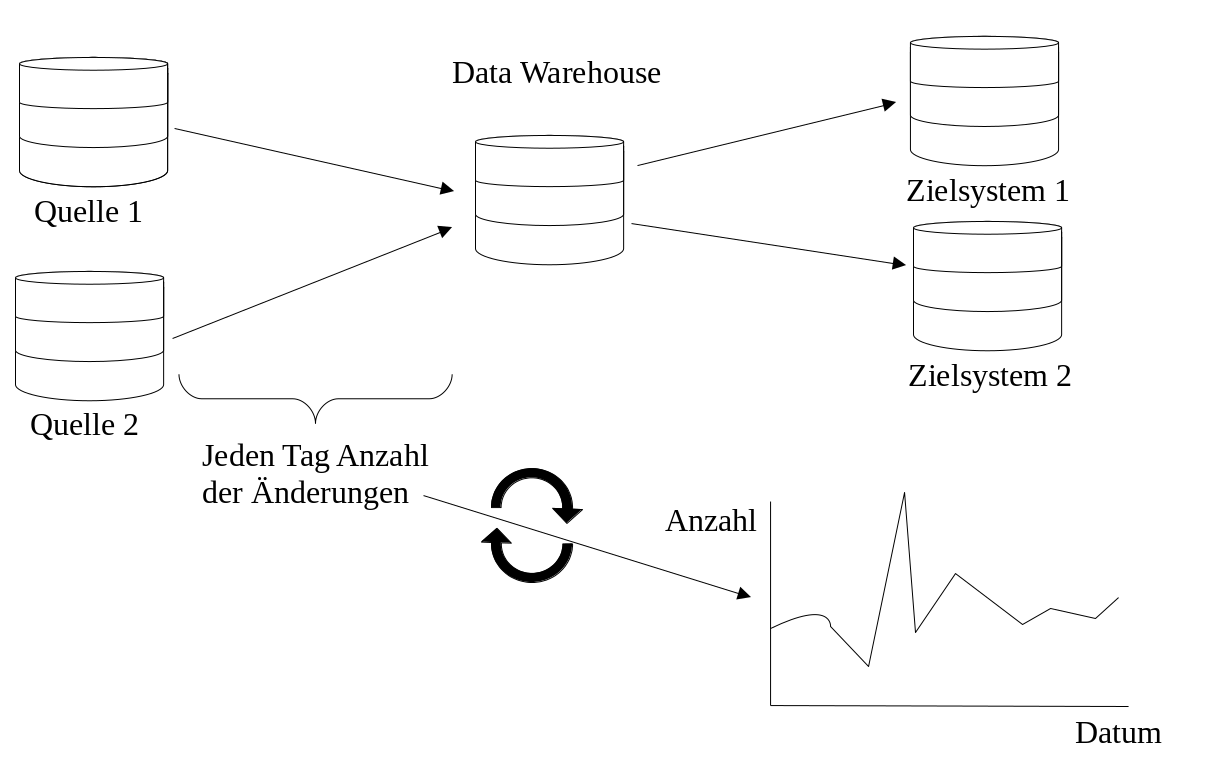
\includegraphics[width=150mm,scale=1]{content/Darstellung_vis_pipeline.png}
\caption{Darstellung des aktuellen Extraktionsverfahrens und Integration der Visualisierung }%
\end{figure}
Die Abbildung zeigt den aktuellen Extraktions-Prozess des Data Warehouse. 
Bei diesem werden Daten aus einigen Quellsystemen abgeholt und in eine zentrale Datenbank, dem Data Warehouse extrahiert.
Anschließend werden die Daten in das korrekte Format konvertiert und den Endsystemen so bereitgestellt, wie diese die Daten erwarten.

Eine mögliche Visualisierung sollte die Meta-Daten, die von den Quellsystemen extrahiert werden erhalten und anschließend visualisieren.
Hierfür wird per Trigger die Daten in Echtzeit an Elastic übertragen, dass die Daten anschließend mit Hilfe eines Kibana Dashboards visualisiert.
Stakeholder sind dann in der Lage grafisch zu sehen, ob es große Abweichungen zu den Monaten / Wochen / Jahren davor gegeben hat und können so einschätzen, ob genauer nachgeforscht werden muss oder ob alles geklappt hat.

%Daten zur Beladung (Delta, Vollbestand) in Echtzeit aus dem DWH nach Elastic exportieren
%-> Anhand eines Dashboards ist es möglich festzustellen, ob es Abweichungen gibt
%-> Ein Experte kann diese Abweichungen dann überprüfen



%Vollständigkeit auf Datensatzebene
%Vollständigkeit auf Attributwerte (es kommen keine null-values hinzu)


%Aktualität die Daten werden schnell genug abgeholt
%Richtigkeit die Daten werden so abgeholt, dass sie fehlerfrei sind

%Ideen:
%- Source und Target vergleichen
%- historisch vergleichen, wie viel zu erwarten ist
%- 

%Die Daten müssen innerhalb einer vorgelegten Range liegen, damit sichergestellt wird, dass die Daten in dem Zielsystem richtig ankommen.



%Zuverlässigkeit, Protokollierung, Dokumentation, Audit der Prozesse
% Verfügbarkeit, Wartbarkeit, Nachvollziehbarkeit







